\chapter{Геометрический метод}
{\bf Вариант №1\\Найти решение задачи линейного программирования геометрически для "а, в, с" на max и min.}

\subsubsection{a)}
\begin{equation*}
    F = x_1 + x_2 \rightarrow max(min)
\end{equation*}
\begin{equation*}
    \begin{cases}
        x_1 + 2x_2 \le 8 \\
        6x_1 - x_2 \le 3 \\
        x_1 \ge 0, x_2 \ge 0
    \end{cases}
\end{equation*}

\begin{center}
    {\bf
    Решение:}
\end{center}

\begin{figure}[ht]
\centering
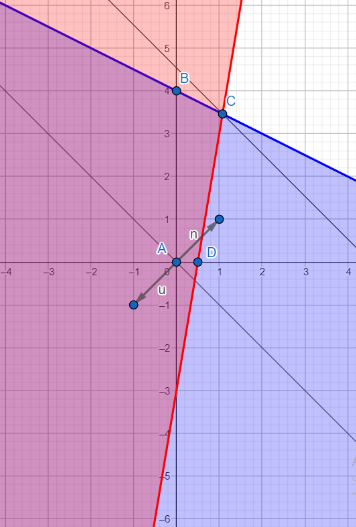
\includegraphics[]{пункт а.png}
\centering
\caption{График для решения задания №1, пункта 1a (построен с помощью \url{https://www.geogebra.org/calculator})}
\end{figure}

\begin{flushleft}
    Синяя область на графике - множество решений 1-го неравенства\\
    Красная область на графике - множество решений 2-го неравенства\\
    Область допустимых значений - четырехугольник ABCD\\
    $\vec{n}\{1; 1\}$ - $\nabla F$ (градиент)\\
    Если перемещать линию уровня (перпендикулярна $\vec{n}$, на графике отмечена серым цветом) в направлении $\vec{n}$, то после прохождения через точку С её пересечение с ОДЗ даёт пустое множество $\implies$ \\С - оптимальная точка задачи максимума\\
    Точка С является пересечением прямых $x_1 + 2x_2 = 8$ и $6x_1 - x_2 = 3 \implies$ координаты точки C являются решением системы:\\
    \begin{equation*}
        \begin{cases}
            x_1 + 2x_2 = 8 \\
            6x_1 - x_2 = 3 \\
        \end{cases}
    \end{equation*}
    Значит $C(\frac{14}{13}; \frac{45}{13}) \implies F_{max} = \frac{14}{13} + \frac{45}{13} = \frac{59}{13}$ \\
    Задача минимума сводится к задаче максимума для функции $G = -F = -x_1 - x_2$ \\
    $\vec{u}\{-1; -1\}$ - $\nabla G$ (градиент)\\
    Если перемещать линию уровня (перпендикулярна $\vec{u}$, на графике отмечена серым цветом) в направлении $\vec{u}$, то после прохождения через точку A её пересечение с ОДЗ даёт пустое множество $\implies$ \\A - оптимальная точка задачи максимума для функции G и, соответственно, задачи минимума для функции F\\
    $A(0; 0) \implies F_{min} = 0 + 0 = 0$
\end{flushleft}

{\bfОтвет:~} $F_{max} = F(\frac{14}{13}; \frac{45}{13}) = \frac{59}{13}$,  $F_{min} = F(0; 0) = 0$ 

\subsubsection{b)}
\begin{equation*}
    F = x_1 + 2x_2 \rightarrow max(min)
\end{equation*}
\begin{equation*}
    \begin{cases}
        x_1 + x_2 \ge 6 \\
        5x_1 - 10x_2 \le 10 \\
        x_1 \ge 0, x_2 \ge 0
    \end{cases}
\end{equation*}

\begin{center}
    {\bf
    Решение:}
\end{center}

\begin{figure}[ht]
\centering
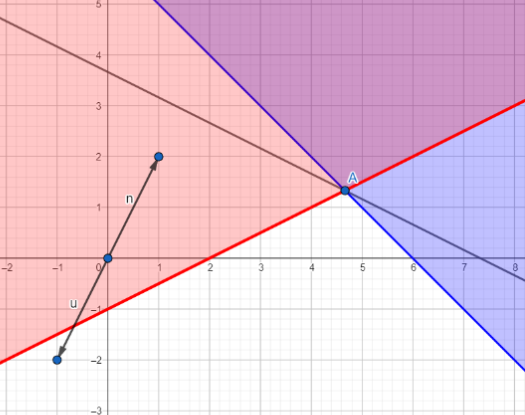
\includegraphics[]{пункт б.png}
\centering
\caption{График для решения задания №1, пункта 1b (построен с помощью \url{https://www.geogebra.org/calculator})}
\end{figure}

\begin{flushleft}
    Синяя область на графике - множество решений 1-го неравенства\\
    Красная область на графике - множество решений 2-го неравенства\\
    Область допустимых значений - часть области пересечения синей и красной областей, лежащая в первом квадранте\\
    $\vec{n}\{1; 2\}$ - $\nabla F$ (градиент)\\
    Область допустимых значений не ограничена в направлении $\vec{n} \implies F_{max}$ не определено\\
    Задача минимума сводится к задаче максимума для функции $G = -F = -x_1 - 2x_2$ \\
    $\vec{u}\{-1; -2\}$ - $\nabla G$ (градиент)\\
    Если перемещать линию уровня (перпендикулярна $\vec{u}$, на графике отмечена серым цветом) в направлении $\vec{u}$, то после прохождения через точку A её пересечение с ОДЗ даёт пустое множество $\implies$ \\A - оптимальная точка задачи максимума для функции G и, соответственно, задачи минимума для функции F\\
    Точка А является пересечением прямых $x_1 + x_2 = 6$ и $5x_1 - 10x_2 = 10 \implies$ координаты точки А являются решением системы:\\
    \begin{equation*}
        \begin{cases}
            x_1 + x_2 = 6 \\
            5x_1 - 10x_2 = 10 \\
        \end{cases}
    \end{equation*}
    Значит $A(\frac{14}{3}; \frac{4}{3}) \implies F_{min} = \frac{14}{3} + 2\cdot\frac{4}{3} = \frac{22}{3}$
\end{flushleft}

{\bfОтвет:~} $F_{max}$ не определено,  $F_{min} = F(\frac{14}{3}; \frac{4}{3}) = \frac{22}{3}$ 



\subsubsection{c)}
\begin{equation*}
    F = x_1 + 2x_2 \rightarrow max(min)
\end{equation*}
\begin{equation*}
    \begin{cases}
        2x_1 - x_2 \ge 6 \\
        2x_1 + x_2 \le 1 \\
        x_1 \ge 0, x_2 \ge 0
    \end{cases}
\end{equation*}

\begin{center}
    {\bf
    Решение:}
\end{center}

\begin{figure}[ht]
\centering
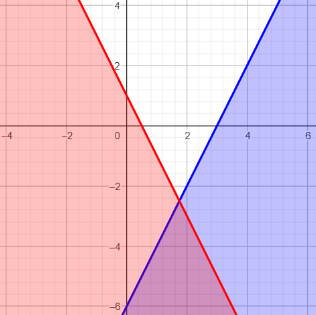
\includegraphics[]{пункт с.png}
\centering
\caption{График для решения задания №1, пункта 1c (построен с помощью \url{https://www.geogebra.org/calculator})}
\end{figure}


\begin{flushleft}
    Синяя область на графике - множество решений 1-го неравенства\\
    Красная область на графике - множество решений 2-го неравенства\\
    Точки, находящиеся в пересечении синей и красной областей, не удовлетворяют условиям $x_1 \ge 0$, $x_2 \ge 0$ $\implies$ область допустимых значений пустая $\implies F_{max}, F_{min}$ не определены
\end{flushleft}

{\bfОтвет:~} $F_{max}, F_{min}$ не определены
